%package list
\documentclass{article}
\usepackage[top=3cm, bottom=3cm, outer=3cm, inner=3cm]{geometry}
\usepackage{multicol}
\usepackage{graphicx}
\usepackage{url}
%\usepackage{cite}
\usepackage{hyperref}
\usepackage{array}
%\usepackage{multicol}
\newcolumntype{x}[1]{>{\centering\arraybackslash\hspace{0pt}}p{#1}}
\usepackage{natbib}
\usepackage{pdfpages}
\usepackage{multirow}
\usepackage[normalem]{ulem}
\useunder{\uline}{\ul}{}
\usepackage{svg}
\usepackage{xcolor}
\usepackage{listings}
\lstdefinestyle{ascii-tree}{
    literate={├}{|}1 {─}{--}1 {└}{+}1 
  }
\lstset{basicstyle=\ttfamily,
  showstringspaces=false,
  commentstyle=\color{red},
  keywordstyle=\color{blue}
}
%\usepackage{booktabs}
\usepackage{caption}
\usepackage{subcaption}
\usepackage{float}
\usepackage{array}

\newcolumntype{M}[1]{>{\centering\arraybackslash}m{#1}}
\newcolumntype{N}{@{}m{0pt}@{}}


%%%%%%%%%%%%%%%%%%%%%%%%%%%%%%%%%%%%%%%%%%%%%%%%%%%%%%%%%%%%%%%%%%%%%%%%%%%%
%%%%%%%%%%%%%%%%%%%%%%%%%%%%%%%%%%%%%%%%%%%%%%%%%%%%%%%%%%%%%%%%%%%%%%%%%%%%
\newcommand{\itemEmail}{schirinosne@unsa.edu.pe}
\newcommand{\itemStudent}{Sebastian Arley Chirinos Negrón}
\newcommand{\itemCourse}{Estructura de datos y Algoritmos}
\newcommand{\itemCourseCode}{1702124}
\newcommand{\itemSemester}{I}
\newcommand{\itemUniversity}{Universidad Nacional de San Agustín de Arequipa}
\newcommand{\itemFaculty}{Facultad de Ingeniería de Producción y Servicios}
\newcommand{\itemDepartment}{Departamento Académico de Ingeniería de Sistemas e Informática}
\newcommand{\itemSchool}{Escuela Profesional de Ingeniería de Sistemas}
\newcommand{\itemAcademic}{2023 - A}
\newcommand{\itemInput}{Del 29 Mayo 2023}
\newcommand{\itemOutput}{Al 05 Junio 2023}
\newcommand{\itemPracticeNumber}{01}
\newcommand{\itemTheme}{Java}
%%%%%%%%%%%%%%%%%%%%%%%%%%%%%%%%%%%%%%%%%%%%%%%%%%%%%%%%%%%%%%%%%%%%%%%%%%%%
%%%%%%%%%%%%%%%%%%%%%%%%%%%%%%%%%%%%%%%%%%%%%%%%%%%%%%%%%%%%%%%%%%%%%%%%%%%%

\usepackage[english,spanish]{babel}
\usepackage[utf8]{inputenc}
\AtBeginDocument{\selectlanguage{spanish}}
\renewcommand{\figurename}{Figura}
\renewcommand{\refname}{Referencias}
\renewcommand{\tablename}{Tabla} %esto no funciona cuando se usa babel
\AtBeginDocument{%
	\renewcommand\tablename{Tabla}
}

\usepackage{fancyhdr}
\pagestyle{fancy}
\fancyhf{}
\setlength{\headheight}{30pt}
\renewcommand{\headrulewidth}{1pt}
\renewcommand{\footrulewidth}{1pt}
\fancyhead[L]{\raisebox{-0.2\height}{
\includegraphics[width=3cm]{img/logo_episunsa.png}}}
\fancyhead[C]{\fontsize{7}{7}\selectfont	\itemUniversity \\ \itemFaculty \\ \itemDepartment \\ \itemSchool \\ \textbf{\itemCourse}}
\fancyhead[R]{\raisebox{-0.2\height}{
\includegraphics[width=1.2cm]{img/logo_abet}}}
\fancyfoot[L]{Sebastian Chirinos Negrón}
\fancyfoot[C]{\itemCourse}
\fancyfoot[R]{Página \thepage}

% para el codigo fuente
\usepackage{listings}
\usepackage{color, colortbl}
\definecolor{dkgreen}{rgb}{0,0.6,0}
\definecolor{gray}{rgb}{0.5,0.5,0.5}
\definecolor{mauve}{rgb}{0.58,0,0.82}
\definecolor{codebackground}{rgb}{72, 0.95, 0.92}
\definecolor{tablebackground}{rgb}{0.8, 0, 0}

\lstset{frame=tb,
	language=bash,
	aboveskip=3mm,
	belowskip=3mm,
	showstringspaces=false,
	columns=flexible,
	basicstyle={\small\ttfamily},
	numbers=none,
	numberstyle=\tiny\color{gray},
	keywordstyle=\color{blue},
	commentstyle=\color{dkgreen},
	stringstyle=\color{mauve},
	breaklines=true,
	breakatwhitespace=true,
	tabsize=3,
	backgroundcolor= \color{codebackground},
}

\begin{document}
	
	\vspace*{10px}
	
	\begin{center}	
		\fontsize{17}{17} \textbf{ Informe de Laboratorio \itemPracticeNumber}
	\end{center}
	\centerline{\textbf{\Large Tema: \itemTheme}}
	%\vspace*{0.5cm}	

	\begin{flushright}
		\begin{tabular}{|M{2.5cm}|N|}
			\hline 
			\rowcolor{tablebackground}
			\color{white} \textbf{Nota}  \\
			\hline 
			     \\[30pt]
			\hline 			
		\end{tabular}
	\end{flushright}	

	\begin{table}[H]
		\begin{tabular}{|x{4.7cm}|x{4.8cm}|x{4.8cm}|}
			\hline 
			\rowcolor{tablebackground}
			\color{white} \textbf{Estudiante} & \color{white}\textbf{Escuela}  & \color{white}\textbf{Asignatura}   \\
			\hline 
			{\itemStudent \par \itemEmail} & \itemSchool & {\itemCourse \par Semestre: \itemSemester \par Código: \itemCourseCode}     \\
			\hline 			
		\end{tabular}
	\end{table}		
	
	\begin{table}[H]
		\begin{tabular}{|x{4.7cm}|x{4.8cm}|x{4.8cm}|}
			\hline 
			\rowcolor{tablebackground}
			\color{white}\textbf{Laboratorio} & \color{white}\textbf{Tema}  & \color{white}\textbf{Duración}   \\
			\hline 
			\itemPracticeNumber & \itemTheme & 04 horas   \\
			\hline 
		\end{tabular}
	\end{table}
	
	\begin{table}[H]
		\begin{tabular}{|x{4.7cm}|x{4.8cm}|x{4.8cm}|}
			\hline 
			\rowcolor{tablebackground}
			\color{white}\textbf{Semestre académico} & \color{white}\textbf{Fecha de inicio}  & \color{white}\textbf{Fecha de entrega}   \\
			\hline 
			\itemAcademic & \itemInput &  \itemOutput  \\
			\hline 
		\end{tabular}
	\end{table}
	
	\section{Tarea}
	\begin{itemize}		
		\item Cree una cuenta de usuario en GitHub usando su correo institucional.
		\item [opcional por ahora] Configure su cuenta de estudiante (https://education.github.com/pack).
		\item Cree un nuevo proyecto personal y desarrolle el ejercicio resuelto en clase. Haga 3 commits como mínimo y muéstrelos. Commit para "¡Hola mundo!", otro para "Bienvenida al curso" y otro para imprimir su nombre.
		\item Cree un proyecto grupal para trabajo colaborativo (de 3 a 5 integrantes).
		\item Cree un archivo por cada tema del manual de java (https://www.w3schools.com/java/default.asp), haga commit e inluyalo en su informe grupal (Dividanse los temas).
		\item Cree ramas para cada integrante y cada cierto tiempo una las ramas al main. No elimine nada para evidenciar ramas, main y commits.

		
	\end{itemize}
		
	\section{Equipos, materiales y temas utilizados}
	\begin{itemize}
		\item Editor Vim
		\item Java
		\item Git
		\item GitHub
		\item C.m. Construye responsablemente soluciones haciendo uso de estructuras de datos y algoritmos, siguiendo un proceso adecuado para resolver problemas computacionales que se ajustan al uso de los recursos disponibles y a especificaciones concretas.
		
	\end{itemize}
	
	\section{URL de Repositorio Github}
	\begin{itemize}
		\item URL del Repositorio GitHub para clonar o recuperar.
		\item \url{https://github.com/BastleyNait/EDA-LAB-B-23A.git}
		\item URL para el laboratorio 04 en el Repositorio GitHub.
		\item \url{https://github.com/BastleyNait/EDA-LAB-B-23A/tree/main/lab01}
	\end{itemize}
	
	\section{Programa en java: Test de iq}

	\subsection{Clase Main}
	\begin{itemize}	
		\item Este un programa Java que utiliza la clase Archivos para leer preguntas de un archivo de texto llamado "TestdeIQ.txt" y permite al usuario ingresar respuestas para cada pregunta. A continuación, se explica el flujo general del programa:
	\end{itemize}	
	
	\lstinputlisting[language=Java, caption={Main.java},numbers=left,]{src/Main.java}	

	\begin{itemize}	
		\item Motrando la Ejecución del codigo:
	\end{itemize}	
	
	\begin{figure}[H]
		\centering
		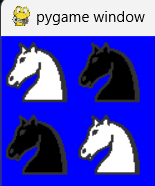
\includegraphics[width=0.3\textwidth,keepaspectratio]{img/Ejercicio2a.png}
		%\includesvg{img/automata.svg}
		%\label{img:mot2}
		%\caption{Product backlog.}
	\end{figure}

%%%%%%%%%%%%%%%%%%%%%%%%%%%%%%%%%%%%%%%%%%%%%%%%%%%%%%%%%%%%%%%%%%%%%%%%%%%%%%%%%%
	\subsection{Ejercicio 02a}
	\begin{itemize}	
		\item Antes de ejecutar el código tenemos que tener en cuenta el importar la función draw del archivo interpreter.py y también todas las funciones de chessPicture:
	\end{itemize}	
	
	\lstinputlisting[language=Python, caption={Ejercicio2a.py},numbers=left,]{src/Ejercicio2a.py}	

	\begin{itemize}	
		\item Motrando la Ejecución del codigo:
	\end{itemize}	
	
	\begin{figure}[H]
		\centering
		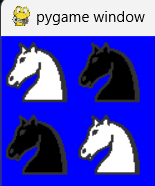
\includegraphics[width=0.3\textwidth,keepaspectratio]{img/Ejercicio2a.png}
		%\includesvg{img/automata.svg}
		%\label{img:mot2}
		%\caption{Product backlog.}
	\end{figure}

		
	\subsection{Estructura de laboratorio 04}
	\begin{itemize}	
		\item El contenido que se entrega en este laboratorio es el siguiente:
	\end{itemize}
	
\begin{lstlisting}[style=ascii-tree]
lab04/
+---EjerciciosDocente
|       defs.py
|       esEscalar.py
|       esPalindromo.py
|       esUnitaria.py
|       numeroPares.py
|       operadoresArit.py
|       pythonClass.py
|       strings.py
|       tablaDeMulti.py
|       test_esEscalar.py
|       test_esUnitaria.py
|       tiposDeDatos.py
|
+---Latex
|   |   .gitignore
|   |   Pweb02_lab04_schirinosne.pdf
|   |   Pweb02_lab04_schirinosne.tex
|   |
|   +---img
|   |       Ejercicio2a.png
|   |       Ejercicio2b.png
|   |       Ejercicio2c.png
|   |       Ejercicio2d.png
|   |       Ejercicio2e.png
|   |       Ejercicio2f.png
|   |       Ejercicio2g.png
|   |       logo_abet.png
|   |       logo_episunsa.png
|   |       logo_unsa.jpg
|   |       pseudocodigo_insercion.png
|   |
|   \---src
|           Ejercicio2a.py
|           Ejercicio2b.py
|           Ejercicio2c.py
|           Ejercicio2d.py
|           Ejercicio2e.py
|           Ejercicio2f.py
|           Ejercicio2g.py
|           Insertion01.java
|           picture.py
|
\---Tarea-del-Ajedrez
        .gitignore
        chessPictures.py
        colors.py
        Ejercicio2a.py
        Ejercicio2b.py
        Ejercicio2c.py
        Ejercicio2d.py
        Ejercicio2e.py
        Ejercicio2f.py
        Ejercicio2g.py
        interpreter.py
        picture.py
        pieces.py
        prueba.py
\end{lstlisting}    

\section{Pregunta: ¿Qué son los archivos *.pyc?}
	\begin{itemize}
		\item Los archivos .pyc son archivos de código compilado en Python. Cuando un archivo fuente de Python (.py) se ejecuta, el intérprete de Python compila ese código en bytecode, que es una representación intermedia del código que puede ser ejecutada más rápido por la máquina virtual de Python. Los archivos *.pyc contienen este bytecode compilado y se generan automáticamente cuando se importa un módulo en Python.
	\end{itemize}	
	\section{Pregunta: ¿Para qué sirve el directorio pycache?}
	\begin{itemize}
		\item El directorio "pycache" es un directorio que se crea automáticamente en Python 3 para almacenar los archivos *.pyc. Cuando se importa un módulo en Python, el intérprete buscará si existe un archivo *.pyc correspondiente en el directorio "pycache". Si lo encuentra y es más reciente que el archivo *.py fuente, el intérprete utilizará el archivo *.pyc en su lugar para ahorrar tiempo de compilación. Si no existe un archivo *.pyc o está desactualizado, el intérprete generará uno nuevo.
	\end{itemize}	
	\section{Pregunta: ¿Cuáles son los usos y lo que representa el subguión en Python?}
	\begin{itemize}
		\item En cuanto al subguión en Python, se le conoce como underscore y se utiliza de diferentes formas:
		\item Nombres de variables especiales: En Python, el subguión se utiliza para nombres de variables especiales que tienen un significado específico. Por ejemplo, un subguión simple se utiliza a menudo como un nombre de variable temporal o como un lugar para ignorar valores que no se necesitan.
		\item Convención para nombres privados: El subguión doble al inicio de un nombre de variable por ejemplo, nombre se utiliza como convención para indicar que un atributo o método es "privado" en Python. No hay verdaderos atributos o métodos privados en Python, pero se considera una convención de estilo no acceder directamente a estos atributos o métodos desde fuera de la clase.
		\item Uso en importaciones: El subguión se utiliza a menudo en las importaciones de módulos en Python.
	\end{itemize}		
	\section{\textcolor{red}{Rúbricas}}
	
	\subsection{\textcolor{red}{Entregable Informe}}
	\begin{table}[H]
		\caption{Tipo de Informe}
		\setlength{\tabcolsep}{0.5em} % for the horizontal padding
		{\renewcommand{\arraystretch}{1.5}% for the vertical padding
		\begin{tabular}{|p{3cm}|p{12cm}|}
			\hline
			\multicolumn{2}{|c|}{\textbf{\textcolor{red}{Informe}}}  \\
			\hline 
			\textbf{\textcolor{red}{Latex}} & \textcolor{blue}{El informe está en formato PDF desde Latex,  con un formato limpio (buena presentación) y facil de leer.}   \\ 
			\hline 
			
			
		\end{tabular}
	}
	\end{table}
	\subsection{\textcolor{red}{Rúbrica para el contenido del Informe y demostración}}
	\begin{itemize}			
		\item El alumno debe marcar o dejar en blanco en celdas de la columna \textbf{Checklist} si cumplio con el ítem correspondiente.
		\item Si un alumno supera la fecha de entrega,  su calificación será sobre la nota mínima aprobada, siempre y cuando cumpla con todos lo items.
		\item El alumno debe autocalificarse en la columna \textbf{Estudiante} de acuerdo a la siguiente tabla:
	
		\begin{table}[ht]
			\caption{Niveles de desempeño}
			\begin{center}
			\begin{tabular}{ccccc}
    			\hline
    			 & \multicolumn{4}{c}{Nivel}\\
    			\cline{1-5}
    			\textbf{Puntos} & Insatisfactorio 25\%& En Proceso 50\% & Satisfactorio 75\% & Sobresaliente 100\%\\
    			\textbf{2.0}&0.5&1.0&1.5&2.0\\
    			\textbf{4.0}&1.0&2.0&3.0&4.0\\
    		\hline
			\end{tabular}
		\end{center}
	\end{table}	
	
	\end{itemize}
	
	\begin{table}[H]
		\caption{Rúbrica para contenido del Informe y demostración}
		\setlength{\tabcolsep}{0.5em} % for the horizontal padding
		{\renewcommand{\arraystretch}{1.5}% for the vertical padding
		%\begin{center}
		\begin{tabular}{|p{2.7cm}|p{7cm}|x{1.3cm}|p{1.2cm}|p{1.5cm}|p{1.1cm}|}
			\hline
    		\multicolumn{2}{|c|}{Contenido y demostración} & Puntos & Checklist & Estudiante & Profesor\\
			\hline
			\textbf{1. GitHub} & Hay enlace URL activo del directorio para el  laboratorio hacia su repositorio GitHub con código fuente terminado y fácil de revisar. &2 &X &2 & \\ 
			\hline
			\textbf{2. Commits} &  Hay capturas de pantalla de los commits más importantes con sus explicaciones detalladas. (El profesor puede preguntar para refrendar calificación). &4 & x&3 & \\ 
			\hline 
			\textbf{3. Código fuente} &  Hay porciones de código fuente importantes con numeración y explicaciones detalladas de sus funciones. &2 &X &2 & \\ 
			\hline 
			\textbf{4. Ejecución} & Se incluyen ejecuciones/pruebas del código fuente  explicadas gradualmente. &2 &X &2 & \\ 
			\hline			
			\textbf{5. Pregunta} & Se responde con completitud a la pregunta formulada en la tarea.  (El profesor puede preguntar para refrendar calificación).  &2 &X &2 & \\ 
			\hline	
			\textbf{6. Fechas} & Las fechas de modificación del código fuente estan dentro de los plazos de fecha de entrega establecidos. &2 &X &2 & \\ 
			\hline 
			\textbf{7. Ortografía} & El documento no muestra errores ortográficos. &2 &X &2 & \\ 
			\hline 
			\textbf{8. Madurez} & El Informe muestra de manera general una evolución de la madurez del código fuente,  explicaciones puntuales pero precisas y un acabado impecable.   (El profesor puede preguntar para refrendar calificación).  &4 &x &4 & \\ 
			\hline
			\multicolumn{2}{|c|}{\textbf{Total}} &20 & &19 & \\ 
			\hline
		\end{tabular}
		%\end{center}
		%\label{tab:multicol}
		}
	\end{table}
	
\clearpage			

\section{Referencias}
\begin{itemize}			
	\item \url{https://www.w3schools.com/python/python_reference.asp}
	\item \url{https://docs.python.org/3/tutorial/}
\end{itemize}	
	
%\clearpage
%\bibliographystyle{apalike}
%\bibliographystyle{IEEEtranN}
%\bibliography{bibliography}
			
\end{document}